\documentclass[a4paper,11pt]{article}
\usepackage[utf8]{inputenc}
\usepackage[english]{babel}
\usepackage[total={18cm,24cm},centering]{geometry}
\usepackage{natbib}
\setcitestyle{super,open={[},close={]}}
\usepackage[colorlinks,citecolor=blue,linkcolor=blue,urlcolor=blue]{hyperref}
\usepackage[pdftex]{graphicx}
\usepackage{tabularx}
\usepackage{textcomp}

\title{\textbf{Effect of Copper on Expression of Functional Genes Associated with {\em Bradyrhizobium
diazoefficiens} Denitrification}}
\author{Pedro J. Pacheco}
\date{}

\begin{document}
\maketitle
\begin{abstract}

Enlace al repositorio: 
\url{https://github.com/pachecopedrojose025/proyecto_final}

Nitrous oxide ($N_2O$) is a powerful greenhouse gas that contributes to climate change.
Denitrification is one of the largest sources of $N_2O$ in soils. The soybean endosymbiont {\em Bradyrhizobium
diazoefficiens} is a model for rhizobial denitrification studies since, in addition to fixing $N_2$, it has
the ability to grow anaerobically under free-living conditions by reducing nitrate from the medium
through the complete denitrification pathway. This bacterium contains a periplasmic nitrate reductase
(Nap), a copper (Cu)-containing nitrite reductase (NirK), a {\em c}-type nitric oxide reductase (cNor), and
a Cu-dependent nitrous oxide reductase (Nos) encoded by the {\em napEDABC}, {\em nirK}, {\em norCBQD} and
{\em nosRZDFYLX} genes, respectively. In this work, the involvement of Cu in growth and denitrification genes expression has been investigated in {\em B. diazoefficiens}. A notable reduction in growth as well as in {\em nirK}, {\em nor} and {\em nos} gene expression  was observed
under oxygen-depleted and Cu-limiting conditions. However, {\em nap} expression was not affected under these conditions. Our results demonstrate,
for the first time, the role of Cu in transcriptional control of {\em B. diazoefficiens}
denitrification. Thus, this study will contribute by proposing useful strategies for reducing $N_2O$
emissions from agricultural soils.
\end{abstract}

\section*{Keywords}
Cu-containing nitrite reductase; enzymatic activity; gene expression; nitric oxide
reductase; nitrous oxide reductase; periplasmic nitrate reductase

\section{Introduction and State of Art}
With a 300-fold greater global warming potential than carbon dioxide ($CO_2$), nitrous
oxide ($N_2O$) is one of the main biogenic greenhouse gases (GHG), and has also been
described as the biggest single cause of ozone depletion \cite{ravishankara2009nitrous}. $N_2O$ emissions from human
activities, fundamentally Agriculture, Forestry and Other Land Use (AFOLU), have notably
increased since the Green Revolution in the early 60s. During the period 2007–2016,
these activities represented 81\% of the anthropogenic emissions of $N_2O$, according to the
last special report by the Intergovernmental Panel on Climate Change \cite{shukla2019climate}. In particular,
agriculture has become the major source of $N_2O$ emissions, accounting for approximately
78\% of the anthropogenic $N_2O$ sources \cite{shukla2019climate} because of a global agricultural intensification
and a great increase in the non-synchronized use of synthetic nitrogen fertilisers \cite{galloway2003nitrogen}\cite{richardson2009mitigating}\cite{taylor2010stoichiometric}.
Several biological pathways occurring in agricultural soils are involved in $N_2O$ emissions.
Among all of them, nitrification and denitrification are the main microbial $N_2O$ sources directly affected by soil nitrogen fertilisation, but only denitrification is known to be the
largest source of $N_2O$ \cite{thomson2012biological}.

Apart from other organisms, such as archaea and fungi, some facultative bacteria
possess the ability to adapt their metabolism to an oxygen-depleted environment in the
presence of nitrate as a respiratory substrate through the activation of denitrification. This
pathway consists of the dissimilatory reduction of nitrate or nitrite to
dinitrogen ($N_2$) via the gaseous intermediates nitric oxide (NO) and nitrous oxide ($N_2O$).
In this process, specific metalloenzymes are sequentially involved: periplasmic (Nap) or
membrane-bound (Nar) nitrate reductases, copper (Cu)-containing (NirK) or cytochrome
${\em cd}_1$-containing (NirS) nitrite reductases, nitric oxide reductases (cNor, qNor or $Cu_ANor$),
and nitrous oxide reductase (Nos). The majority of denitrifiers are found in the phylum
Proteobacteria, within the domain Bacteria. The alpha-proteobacterium {\em Paracoccus denitrificans}
and the 
gamma-proteobacteria {\em Pseudomonas stutzeri} and {\em Pseudomonas aeruginosa} are the
first model organisms where denitrification were widely studied. Reviews covering the
physiology, biochemistry and molecular genetics of denitrification have been published
elsewhere \cite{zumft1997cell}\cite{vannitrogen}\cite{van2007introduction}\cite{kraft2011microbial}\cite{bueno2012bacterial}\cite{torres2016nitrous}.Over recent years, several reports about denitrification in plant endosymbiotic
bacteria emerged \cite{bedmar2005complete}\cite{bedmar2013ecology}\cite{salas2021bacterial}. Thanks to their capacity to establish a $N_2$-fixing symbiotic
relationship with plants, these bacteria can contribute to natural N soil enrichment, while
reducing the need for chemical fertilisation. Therefore, symbiotic $N_2$ fixation is considered a
process with economic, ecological and agricultural importance. In this process, a mutualist
association between soil bacteria, commonly known as rhizobia, and plants of the Fabaceae
family is established. Rhizobia may induce the formation of nodules in the legume roots
and on the stems of some aquatic legumes; nodules are specialized structures where $N_2$
fixation takes place \cite{poole2018rhizobia}.

{\em Bradyrhizobium diazoefficiens}, which establishes nitrogen-fixation symbiosis with soybean
({\em Glycine max}), is considered a model organism in the study of denitrification in
rhizobia because it is the only known rhizobia species able to grow under oxygen-limiting
conditions with nitrate as sole electron acceptor and, also, to perform the complete denitrification
pathway under both free-living and symbiotic conditions \cite{bedmar2005complete}. Denitrification
in {\em B. diazoefficiens} is carried out by a periplasmic nitrate reductase (Nap), encoded by the
{\em napEDABC} operon \cite{delgado2003bradyrhizobium}, a Cu-containing nitrite reductase (NirK), encoded by the {\em nirK}
gene \cite{velasco2001characterization}, a cytochrome {\em c}-type nitric oxide reductase (cNor), encoded by the {\em norCBQD}
operon \cite{mesa2002characterization}, and a Cu-dependent nitrous oxide reductase (Nos), encoded by the {\em nosRZDFYLX}
genes \cite{velasco2004molecular}. Nap is a functional heterodimer comprising the catalytic subunit NapA of
about 90 kDa that contains a bis molybdopterin guanine dinucleotide ($Mo[MGD]_2$) cofactor
and a [4Fe-4S] centre, and NapB (15 kDa) that contains 2 heme {\em c} groups and receives
electrons from the membrane-bound NapC (25 kDa) which binds 4 heme {\em c} groups. NirK
is a homotrimer with a predicted molecular mass of about 35 kDa per monomer that
contains type 1 and type 2 Cu centres. The catalytic subunit of cNor, NorB, contains heme {\em b}
and a binuclear active centre (heme ${\em b}_3$ and $Fe_B$). NorC is a membrane-anchored protein
(16 kDa) that contains heme {\em c}. Finally, the catalytic subunit of Nos, NosZ (120–160 kDa), is
a homodimer Cu-containing enzyme with two distinct Cu centres ($Cu_A$ and $Cu_Z$).

Similarly to many other denitrifiers, expression of denitrification genes in {\em B. diazoefficiens}
requires both oxygen limitation and the presence of nitrate or a derived nitrogen oxide
(NOx), this control being mediated by the FixLJ-$FixK_2$-NnrR regulatory cascade \cite{mesa2003bradyrhizobium}\cite{mesa2008comprehensive}\cite{bueno2017disparate}.
In fact, the expression of {\em napEDABC}, {\em nirK} and {\em nosRZDFYLX} genes requires microoxic
conditions and directly depends on the transcriptional regulator $FixK_2$ \cite{bueno2017disparate}\cite{torres2017fixk2}, while expression
of {\em norCBQD} genes relies on NO, being NnrR the transcriptional regulator which
directly interacts with the {\em norCBQD} promoter \cite{bueno2017disparate}\cite{jimenez2019expanding}. In this context, the molecular discriminatory
determinants for selective $FixK_2$ recognition and target activation were recently unveiled \cite{cabrera2021dissection}.

Besides being a source of $N_2O$, the ecological and environmental importance of denitrification
lies in the fact that Nos is the only known enzyme able to remove $N_2O$ from
ecosystems \cite{richardson2009mitigating}, the expression and activity of this enzyme becoming a natural target to effectively reduce $N_2O$ emissions from agricultural soils. Increasing knowledge of the regulation
and biochemistry of $N_2O$ metabolism in rhizobia will raise opportunities for the design of effective mitigation strategies to reduce $N_2O$ emissions from legume crops \cite{bakken2017sources}.

Nowadays, new environmental factors are emerging as candidates for controlling
denitrification, such as pH \cite{carreira2020effect}\cite{olaya2021effect} or Cu \cite{black2016influence}. In the case of Cu, it is an essential cofactor in
critical enzymes, such as multicopper oxidases, as well as the Nos and NirK denitrification
enzymes. The role of this metal in denitrification has been studied in a wide range of
non-symbiotic microorganisms, such as {\em Pseudomonas perfectomarinus} \cite{matsubara1982modulation}, {\em P. stutzeri} \cite{black2016influence},
{\em P. denitrificans} \cite{felgate2012impact}\cite{sullivan2013copper} and {\em Achromobacter xylosoxidans} \cite{felgate2012impact}. Regarding rhizobia, Serventi et al.
(2012) \cite{serventi2012copper} investigated the role of Cu in cytochrome oxidase biogenesis in {\em B. diazoefficiens}.
Nevertheless, studies covering Cu influence on the denitrification pathway in rhizobia are
scarce. In this study, the effect of different Cu regimes on growth and gene expression is analysed in free-living cultures.

\section{Materials and Methods}
\subsection{Bacterial strains and growth conditions}
Bacterial strains used in this study are compiled in Table \ref{tab:table1}. 

\begin{table}[h!]
\centering
\caption{{\em B. diazoefficiens} strains used in this study.}
\begin{tabular}{|c|c|c|}
\hline
\textbf{Strains} & \textbf{Relevant description} & \textbf{Reference} \\
\hline
110spc4 & Wild-type & \cite{regensburger1983rna} \\
\hline
BG0602 & {\em napE-lacZ} fusion-containing strain & \cite{robles2006bradyrhizobium} \\
\hline
RJ2498 & {\em nirK-lacZ} fusion-containing strain & \cite{mesa2003bradyrhizobium} \\
\hline
RJ2499 & {\em norC-lacZ} fusion-containing strain & \cite{mesa2003bradyrhizobium} \\
\hline
BG0301 & {\em nosR-lacZ} fusion-containing strain & \cite{torres2017fixk2}\\
\hline
\end{tabular}
\label{tab:table1}
\end{table}

{\em B. diazoefficiens}
cells were cultivated routinely under oxic conditions at 30\textcelsius in peptone–salts–yeast extract
(PSY) medium supplemented with 0.1\% L-arabinose, essentially as described by Mesa et al.
(2008) \cite{mesa2008comprehensive}. Buffered Vincent’s minimal medium, here defined as vitamin-free modified
Vincent’s minimal medium (BVM, \cite{vincent1970manual}\cite{becker2004global}) was used in this study, containing the following
ingredients (per litre): $KH_2PO_4$, 2 g; $K_2HPO_4$, 2 g; $NH_4Cl$, 840 mg; $MgSO_4$, 246.48 mg;
$CaCl_2$, 67.63 mg; $FeCl_3$, 10 mg; MOPS, 2.09 g. This medium was supplemented
with 3 g of 1 M arabinose and 1 mL from a mineral solution \cite{bishop1976relation} consisting of: $H_3BO_3$,
145 mg; $ZnSO_4$, 108 mg; $Na_2MoO_4$, 125 mg; $MnCl_2$, 4 mg; $FeSO_4$,
125 mg; $CoSO_4$, 70 mg; nitrile triacetate, 7 g; $CuSO_4$, 5 mg. When needed, the
medium was supplemented with 10 mM $KNO_3$ (referred here as BVMN). Final pH was
adjusted around 6.8 with 2 M $NH_3$.

Final Cu concentration in BVM or BVMN as indicated in the original recipe \cite{vincent1970manual} was
0.02 $\mu$M, referred to in this manuscript as Cu-standard medium (Cu-S). In this study, 13 $\mu$M
Cu was used as high Cu conditions (Cu-H); this concentration was also used as Cu-H in
previous studies \cite{felgate2012impact}\cite{sullivan2013copper}. In the case of the Cu-limiting medium (Cu-L), $CuSO_4$ was
omitted from the mineral solution, and 10 $\mu$M bathocuproine disulfonic acid (BCS) (Cu(I)
chelator) and 1 mM L-ascorbate (reducer from Cu(II) to Cu(I)) were added to the medium
in order to lower Cu availability \cite{felgate2012impact}\cite{serventi2012copper}. Only for the Cu-L medium, glassware was treated
overnight with 0.1 M HCl and rinsed afterwards with double-distilled water \cite{serventi2012copper}.

After growing under oxic conditions in the PSY medium, {\em B. diazoefficiens} cells were
collected by centrifugation (8000 g, 8 min, 4\textcelsius). Next, cells were washed twice with BVM
or BVMN and inoculated at an optical density at 600 nm ($OD_{600}$) of 0.05 (or 0.2 when needed). For oxic conditions,
3 mL of medium were added to 17-mL tubes. For anoxic conditions, 17-mL tubes were
completely filled with medium. For microoxic conditions, 3, 50 and 100 mL of medium were added to 17-mL, 250 and 500-mL rubber stoppered tubes or Erlenmeyer flasks, respectively.
The headspace was then filled with a gas mixture consisting of 2\% (v/v) oxygen and 98\% (v/v)
$N_2$ and both, tubes and flasks, were incubated at 30\textcelsius with agitation at 170 rpm.

When needed, antibiotics were added to {\em B. diazoefficiens} cultures at the following
concentrations ($\mu$g/mL): spectinomycin (Spc), 200 (solid cultures), 100 (liquid cultures);
streptomycin (Sm), 200 (solid cultures), 100 (liquid cultures); tetracycline (Tc), 100 (solid
cultures), 25 (liquid cultures); kanamycin (Km), 200 (solid cultures), 100 (liquid cultures);
chloramphenicol (Cm), 20.

\subsection{Determination of $\beta$-galactosidase activity}
$\beta$-galactosidase activity was analysed using permeabilised cells from at least three
independent cultures (3 mL), assayed in triplicate for each strain and condition, as previously
described \cite{cabrera2016integrated}. Specific activity was calculated in Miller Units \cite{miller1972miller} applying the formula shown in (\ref{eq:equation1}):

\begin{equation}
\label{eq:equation1}
U=[1000*(OD_{420}-OD_{550})]/[t(min)*V(mL)*OD_{595}]
\end{equation}

where:

OD420 y OD550 are the optical density values of the reaction,

OD595 is the optical density of the culture used in the reaction,

t is the time of incubation of all the reactions, always expressed in minutes,

and V is the volume of the reaction, always expressed in mL.


$\beta$-galactosidase activity in the presence of NO was analyzed by generating this gas chemically according
to Bricio et al. (2014) \cite{bricio2014third} and adding (50 $\mu$M final concentration) to the tubes 5 h before
activity measurements.

\subsection{Analysis of gene expression by qRT-PCR}
Expression of {\em napE}, {\em nirK}, {\em norC} and {\em nosR} was analysed by qRT-PCR using a QuantStudio
3 Real-Time PCR system (Thermo Fisher Scientific,Waltham, MA, USA). {\em B. diazoefficiens}
110spc4 was grown microaerobically in the BVMN medium under Cu-L or Cu-S conditions
for 48 h. Cell harvest, isolation of total RNA and cDNA synthesis were performed as
described previously \cite{mesa2003bradyrhizobium}. Primers for the PCR reactions were specifically designed
with the Clone Manager Suite software to have melting temperatures between 57\textcelsius and
62\textcelsius and generate PCR products of 75–100 bp. Each PCR reaction contained 9.5 $\mu$L of
iQTM SYBR Green Supermix (Bio-Rad, Hercules, CA, USA), 2 mM (final concentration) of
individual primers and appropriate dilutions of different cDNA samples in a total volume
of 19 $\mu$L. Reactions were run in triplicate. Melting curves were generated to verify the
specificity of the amplification. Relative changes in gene expression were calculated as
described by Pfaffl (2001) \cite{pfaffl2002relative}. Expression of the 16S {\em rrn} gene was used as reference for
normalization (Table \ref{tab:table2}).

\begin{table}[h!]
\centering
\caption{{\em B. diazoefficiens} strains used in this study.}
\begin{tabular}{|c|c|}
\hline
\textbf{Primers} & \textbf{DNA sequence 5'-3'} \\
\hline
bsr7036({\em napE})-for4 & GCCTTCCTGTTCCTGAC \\
\hline
bsr7036({\em napE})-rev4 & CCGGCAAACATCTGGTAGA \\
\hline
{\em nirK}-6for & AGCCTTCACCGACACCGAAGAG \\
\hline
{\em nirK}-6rev & GAGCGCATTCTTGCCGGTAAGC \\
\hline
{\em norC}-3for & GCAGATGCCGCAGTTCAAC \\
\hline
{\em norC}-3rev & TGATCGTGCTCACCCATTG \\
\hline
{\em nosR}-for & ATGATCCAGGTGCGGCTGAAG \\
\hline
{\em nosR}-rev & CCGGCTGTGATGATTGTGTTCG \\
\hline
16S-for & GCAGGCTTAACACATGCAAGTC \\
\hline
16S-rev & AGGTACGTTCCCACGCGTTACTC \\
\hline
\end{tabular}
\label{tab:table2}
\end{table}

\subsection{Statistical analysis}
The total number of replicates is given in each figure. Data were checked for normal
distribution according to Kolmogorov–Smirnov and Shapiro–Wilk tests. We then performed
inferential statistics to test null hypotheses applying a parametric ANOVA for unpaired
treatments. Next, a post-hoc Tukey HSD test at $p<0.05$ with SPSS software was performed.

\section{Results}
\subsection{Cu effect on {\em B. diazoefficiens} 110spc4 growth under different oxygen conditions}
{\em B. diazoefficiens} 110spc4 was grown under oxic, anoxic and microoxic (2\% initial $O_2$
concentration) conditions in Buffered Vincent’s medium \cite{serventi2012copper} supplemented with nitrate
(BVMN) and different Cu concentrations: Cu limitation, {\em i.e.}, chelated (Cu-L), Cu standard
(Cu-S, 0.02 $\mu$M) or high Cu (Cu-H, 13 $\mu$M) (Figure \ref{fig:figure1}). Under oxic conditions, cultures
reached an optical density at 600 nm ($OD_600$) of around 1.5 after 7 days of incubation,
regardless of the Cu treatment (Figure \ref{fig:figure1}A). These results suggest that Cu was not a limiting
factor for {\em B. diazoefficiens} growth by oxygen respiration (Figure \ref{fig:figure1}A). 
\begin{figure}[h!]
\centering
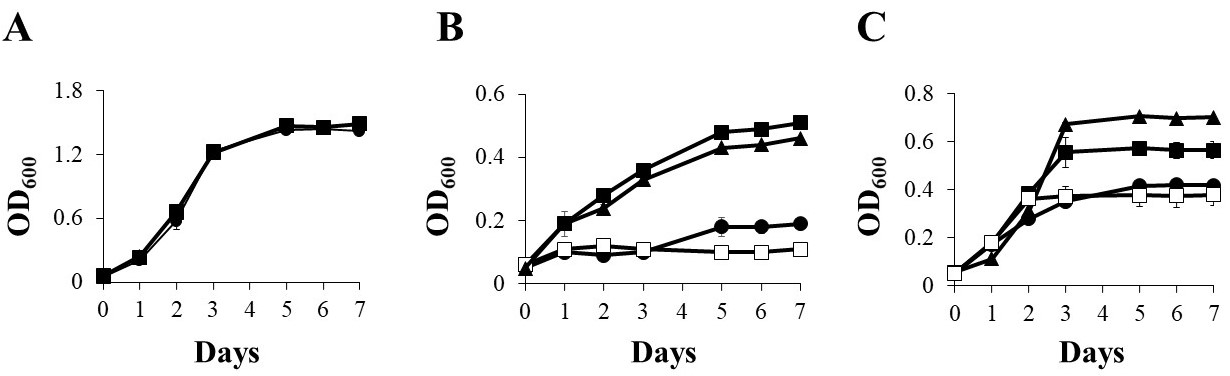
\includegraphics[height=5cm]{Images/Figure1.jpg}
\caption{Growth of {\em B. diazoefficiens} 110spc4 in Cu limitation (Cu-L) (black circle), Cu standard (Cu-S) (black square) and
high Cu (Cu-H) (black triangle) BVMN media under oxic (A), anoxic (B) and microoxic (C) conditions. In (B,C),
growth in the Cu-S BVM medium was also included (white square). Error bars represent standard error between
triplicates, and where not visible, these were smaller than the symbols}.
\label{fig:figure1}
\end{figure}

When {\em B. diazoefficiens} 110spc4 cells were cultured in BVMN medium under anoxic
conditions (Figure \ref{fig:figure1}B), Cu-L cultures reached a turbidity ($OD_{600}$) of about 0.2 after 7 days
of incubation, while Cu-S and Cu-H cultures reached an $OD_{600}$ of about 0.5, indicating that
growth was severely affected in the Cu-L medium compared with Cu-S or Cu-H media
(Figure \ref{fig:figure1}B). This result indicates that Cu was essential for nitrate-dependent anaerobic
growth of {\em B. diazoefficiens}. In fact, the growth profile displayed in BVMN Cu-L cultures
with nitrate was similar to that observed in Cu-S cultures incubated without nitrate (BVM
medium) (Figure \ref{fig:figure1}B), indicating that Cu and nitrate were both indispensable for nitrate
respiration under anoxic conditions. Finally, {\em B. diazoefficiens} 110spc4 cells were incubated
under microoxic conditions in Cu-L, Cu-S and Cu-H BVMN media. As shown in Figure \ref{fig:figure1}C,
microaerobic growth under Cu-L conditions decreased compared with that reached under
Cu-S conditions (about 0.4 and 0.6 $OD_{600}$, respectively, after 7 days of incubation). In
contrast, cells grown in the Cu-H medium showed a significant increase in growth rates
compared with those cultured in the Cu-S medium (about 0.7 and 0.6 $OD_{600}$, respectively,
after 7 days of incubation). Interestingly, when cells were grown microaerobically in the Cu-S medium, but in the absence of nitrate, they displayed similar growth rates to
those cultured in Cu-L conditions with nitrate as the respiratory substrate (Figure \ref{fig:figure1}C).
These results suggest that nitrate and Cu were necessary for {\em B. diazoefficiens} to grow from
nitrate respiration under microoxic conditions, as it was observed under anoxic conditions
(Figure \ref{fig:figure1}B).

\subsection{Disparate response of denitrification gene expression to Cu}
Taking the previous results into consideration, we decided to perform a study into the Cu
effect on denitrification gene expression, by incubating cells for 3 days under different Cu
concentrations. For this purpose, we analysed $\beta$-galactosidase activity from the {\em napE-lacZ},
{\em nirK-lacZ}, {\em norC-lacZ} and {\em nosR-lacZ} transcriptional fusions in {\em B. diazoefficiens} 110spc4 cells
grown for 3 days in Cu-L, Cu-S and Cu-H BVMN media, under microoxic conditions
(Figure \ref{fig:figure2}). Cultures grown aerobically were included as a control in the experiments. As
shown in Figure \ref{fig:figure2}A, {\em napE-lacZ} microaerobic expression was not significantly affected by
Cu concentration in the medium, demonstrating similar $\beta$-galactosidase activity values
under Cu-L, Cu-S or Cu-H conditions. These results indicate that Cu is not involved
in the transcriptional control of {\em napEDABC} genes. In contrast, Cu limitation drastically
lowered $\beta$-galactosidase activity from the {\em nirK-lacZ}, {\em norC-lacZ} and {\em nosR-lacZ} fusions (about
3-, 6- and 4-fold, respectively) compared with the values obtained in the Cu-S medium
(Figure \ref{fig:figure2}B–D). These results suggest that Cu availability is essential for {\em nirK}, {\em norCBQD}
and {\em nosRZDFYLX} maximal expression.

\begin{figure}[h!]
\centering
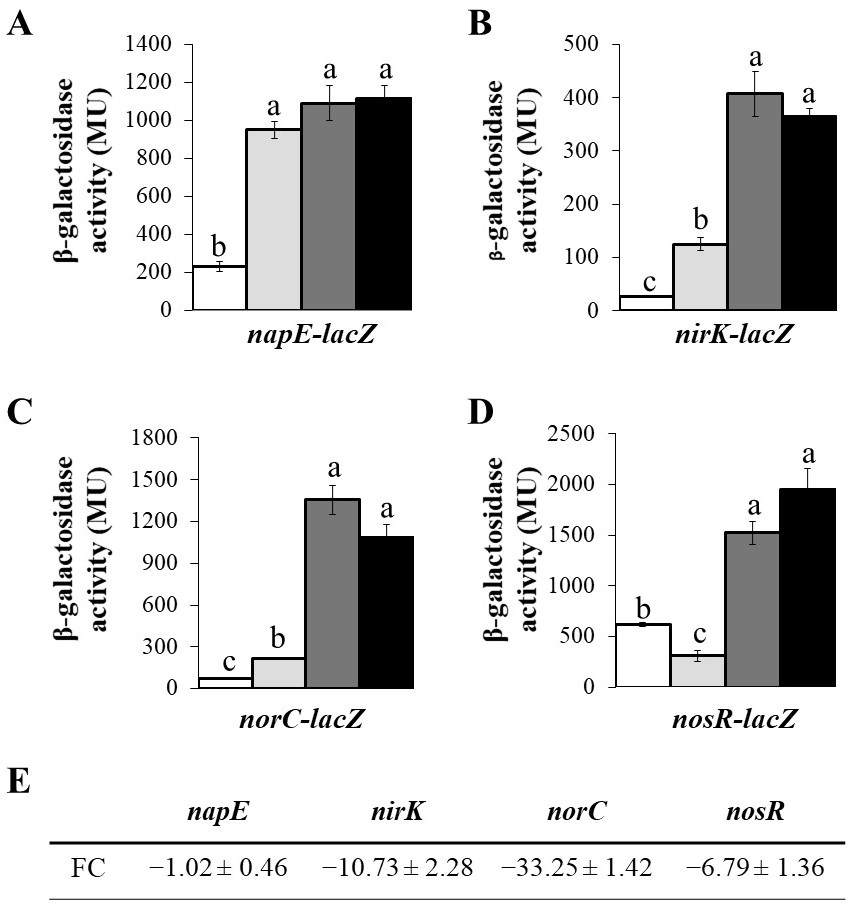
\includegraphics[height=13cm]{Images/Figure2 (2).jpg}
\caption{Transcriptional expression of denitrification genes monitored as $\beta$-galactosidase activity
from {\em napE-lacZ} (A), {\em nirK-lacZ} (B), {\em norC-lacZ} (C) and {\em nosR-lacZ} (D) fusions chromosomally integrated
in {\em B. diazoefficiens} 110spc4 grown aerobically in Cu-S (white bars) and microaerobically in Cu-L (light
grey bars), Cu-S (dark grey bars) and Cu-H (black bars) BVMN media for 3 days. A post-hoc Tukey
HSD test at $p<0.05$ was applied in (A–D); same lower-case letters in each figure indicate that
values are not statistically different. (E) Expression changes of {\em napE}, {\em nirK}, {\em norC} and {\em nosR} genes in
{\em B. diazoefficiens} 110spc4 grown microaerobically in Cu-L compared with Cu-S measured by qRT-PCR.
Data expressed as Miller Units (MU) and Fold Change (FC) are means with standard deviation from
at least three independent cultures assayed in triplicate.}
\label{fig:figure2}
\end{figure}

The negative effect of Cu limitation on {\em nirK}, {\em nor} and {\em nos} transcriptional expression was also confirmed by qRT-PCR analyses. When cells were cultured microaerobically in
the Cu-L BVMN medium, expression of {\em nirK}, {\em norC} and {\em nosR} genes was reduced to 10.73,
33.25 and 6.79, respectively, compared with that observed in cells cultured in the Cu-S
medium (Figure \ref{fig:figure2}E). In contrast, Cu limitation did not affect {\em napE} expression compared
with Cu-S conditions, similar to the results obtained when we analysed the {\em napE-lacZ}
transcriptional fusion (Figure \ref{fig:figure2}A,E). Taken together, these results confirm the negative
effect of Cu limitation on {\em nirK}, {\em nor} and {\em nos} but not on {\em nap} gene expression.

\section{Discussion}
The main focus of the present work was to contribute to a better understanding of the
role of Cu in {\em B. diazoefficiens} denitrification. To achieve this goal, we undertook a
study of the expression of the {\em nap}, {\em nirK}, {\em nor} and {\em nos} genes involved in the denitrification pathway. Firstly, we analysed the capacity of
{\em B. diazoefficiens} 110spc4 to grow under different Cu conditions: Cu limitation (Cu-L), Cu
standard (Cu-S) or high Cu (Cu-H). Aerobic growth was not affected by Cu limitation
indicating that Cu-independent terminal oxidases can function under these conditions. In
fact, like other aerobic facultative bacteria, {\em B. diazoefficiens} adapts its metabolism to different
oxygen conditions through the expression of multiple terminal oxidases with a distinct
affinity for oxygen \cite{delgado1998genes}. Eight terminal oxidases have been identified in {\em B. diazoefficiens},
of which two are Cu-independent {\em bd}-type oxidases, and the remaining six are heme-
Cu oxidases, which use Cu as cofactor \cite{buhler2010disparate}. It might be possible that {\em bd}-type oxidases
are responsible for the aerobic growth under Cu limitation. As reviewed by Jünemann
(1997) \cite{junemann1997cytochrome}, the expression of cytochrome {\em bd} increased concomitantly with oxygen depletion
in {\em E. coli}; however, major expression levels of this type of cytochrome were observed with
the increase in oxygen concentration in {\em Azotobacter vinelandii}. In the Gram-positive human
pathogenic bacterium {\em Mycobacterium tuberculosis}, Cu-independent cytochrome {\em bd} oxidases
were induced under hypoxia, decreasing Cu requirement as a consequence, which is
beneficial for the bacterium because Cu toxicity rises under these conditions \cite{marcus2016csor}. Therefore,
an adaptation to oxic Cu-depleted conditions through the synthesis of Cu-independent
oxidases in {\em B. diazoefficiens} would be a plausible hypothesis for the observed phenotype.

In contrast to oxic conditions, Cu limitation negatively affected anaerobic and microaerobic
nitrate-dependent growth. However, other denitrifiers, such as {\em P. denitrificans}
or {\em A. xylosoxidans} did not show significant growth differences between Cu-L and Cu-H
media under anaerobiosis with nitrate as the respiratory substrate \cite{felgate2012impact}. The presence of
the Cu-independent NirS in {\em P. denitrificans} could explain the growth differences under
Cu-L conditions between this bacterium and {\em B. diazoefficiens}. However, {\em A. xylosoxidans}
that, similarly to {\em B. diazoefficiens}, possesses a Cu-dependent NirK, was also able to grow
anaerobically in a Cu-limiting medium \cite{felgate2012impact}. These different results could be explained
by the different growth conditions used in our work and in the aforementioned study,
where both {\em A. xylosoxidans} and {\em P. denitrificans} were grown as continuous cultures in a
chemostat. Another possible explanation for these differences could be given by the fact
that both {\em A. xylosoxidans} and {\em P. denitrificans} are rapid-growing microorganisms \cite{felgate2012impact}, while
{\em B. diazoefficiens} is a slow-growing bacterium. The slow growth rate of {\em B. diazoefficiens} might
have contributed to the negative effect of Cu limitation on the expression and activation of
the complete denitrification machinery, and this could be a possible reason for the growth
defects observed in Cu-L compared with Cu-S and Cu-H. Contrary to the results observed
in this work, Sullivan et al. (2013) \cite{sullivan2013copper} did not observe any growth difference between
Cu-L and Cu-H in {\em P. denitrificans} batch cultures. The lack of a growth defect observed
in {\em P. denitrificans} under Cu-L conditions \cite{sullivan2013copper} compared with {\em B. diazoefficiens} could also
be explained by the fact that the denitrification process starts by a membrane-bound nitrate
reductase (Nar) in {\em P. denitrificans}, and by a periplasmic nitrate reductase (Nap) in
{\em B. diazoefficiens}. Recent evidence supporting this idea was reported in {\em P. stutzeri}, another
rapid-growing microorganism in which the denitrification process also begins with the
reduction of nitrate to nitrite by a Nar \cite{black2016influence}. In the latter study, no significant differences in
growth were observed in anaerobic cultures of {\em P. stutzeri} over a 7-day period throughout a
Cu concentration range between 0 and 1 mM Cu. Therefore, our work provides evidence
that Cu limitation could affect growth of slow-growing microorganisms provided with
both a Nap as the first enzyme of the denitrification process and a Cu-dependent NirK.

To better understand the effect of Cu on {\em B. diazoefficiens} denitrification, we investigated
gene expression in microaerobic Cu-L, Cu-S and Cu-H cultures. By using transcriptional fusions to the reporter gene {\em lacZ}, we demonstrated the Cu dependence of {\em nirK}, {\em nor} and {\em nos} denitrification
gene induction under microoxic conditions. These observations were confirmed by
performing qRT-PCR analyses of the {\em napA}, {\em nirK}, {\em norC} and {\em nosR} genes. Similarly to our
observations, adequate bioavailable Cu concentrations (0.15 mM) resulted in the greatest
transcription levels of {\em P. stutzeri} {\em nirS}, {\em norB} and {\em nosZ} denitrification genes compared with
low Cu \cite{black2016influence}. Moreover, low levels of {\em nosZ} expression during Cu limitation were also
reported in {\em P. denitrificans} \cite{sullivan2013copper}.

Gene expression results clearly indicated that the induction of {\em nirK}, {\em nor} and {\em nos} genes
by low oxygen and nitrate was significantly reduced under Cu limitation, suggesting
that this control might be modulated by a specific repressor. In this context, CsoR and
CopY are considered as Cu-sensing transcriptional ATPase repressors in bacteria, such
as {\em M. tuberculosis} \cite{liu2007csor}, {\em E. coli} and {\em Enterococcus hirae} (for a review, see Rademacher and
Masepohl, 2012 \cite{rademacher2012copper}). Nevertheless, a {\em csoR}-{\em cueA} divergon encoding a CsoR-like repressor
and a heavy metal transporting P-type ATPase (CueA) was recently reported in the
Gram-negative bacterium {\em Bradyrhizobium liaoningense} CCNWSX0360 \cite{liu2007csor}. These authors
attributed a crucial role in Cu homeostasis to this system, as well as in zinc/cadmium resistance.
A search of the {\em B. diazoefficiens} genome in the KEGG database (\url{https://www.genome.
jp/kegg/}) revealed the presence of a putative gene encoding a
repressor from the CsoR family whose annotation is bsr0701. Apart from the probable role
of this repressor in metal tolerance, a putative role of the predicted CsoR protein in the
low transcription levels of {\em B. diazoefficiens} {\em nirK}, {\em nor} and {\em nos} under Cu limitation requires
further investigation.

\section{Conclusions}
The main goal of the present work was to investigate the influence of Cu on denitrification
in the soybean endosymbiont {\em B. diazoefficiens}. Taken together, our results suggest that
Cu may
act as an essential factor in the regulation of the denitrification gene expression. Therefore, Cu could be involved in the denitrification regulatory network and
not only acts as a mere enzymatic cofactor of the Cu-dependent enzymes, but also as an
important regulatory signal of this process.

\bibliographystyle{unsrt}
\bibliography{references.bib}

\end{document}  